%%%%%%%%%%%%%%%%%%%%%%%%%%%%%%%%%%%%%%%%%%%%%%%%
\chapter{Weeks}
%%%%%%%%%%%%%%%%%%%%%%%%%%%%%%%%%%%%%%%%%%%%%%%%
Title: Java Mode for Simulating Native Image Behaviour

Description: GraalVM Native Image compiles Java programs into native binaries that operate under the closed-world assumption. This means that every reflectively-accessed element such as Class, Executable, or Field must be provided as reachability metadata to the image-build process. In Native Image, the reachability metadata is either 1) provided via user-provided configuration files in JSON format or 2) computed by partially evaluating the input program to pre-compute the reflectively-accessed elements.
Due to the long image-build times, creating the correct metadata can be a time-consuming process for users: if the metadata for any element is missing, the entire image needs to be rebuild.
The objective of this project is to allow users to compute metadata with a quick turnaround by introducing a new mode to the JDK, so that it operates under the closed-world assumption and behaves exactly like Native Image.
We modify all reflective JDK features to operate under a closed-world assumption by checking the reachability metadata to determine if the reflectively accessed element is in the closed world. To pre-compute the reflectively-accessed elements we implement a bytecode-to-bytecode partial evaluator that transforms classes before they are loaded and extracts reachability metadata from them.
%%%%%%%%%%%%%%%%%%%%%%%%%%%%%%%%
\section{Week 1 - 18.09.23}
%%%%%%%%%%%%%%%%%%%%%%%%%%%%%%%%

%%%%%%%%%%%%%%%%
\subsection{Meeting Vojin - 18.09}
%%%%%%%%%%%%%%%%
do restriction on java, and need to specify them, some hacky stuff is also introduced, introduce plugin to say how the restrictive image should work.
first build java, try to modify

Restrictions:
- java.lang.System#getSecurityManager returns null
- java.lang.ClassLoader#defineClass[0|1|2] throws unsupported operation exception → native are package protected throws unsupported operation exception
- “java.home” in com.oracle.svm.core.jdk.SystemPropertiesSupport (find what we change and introduce it into java) \url{https://github.com/oracle/graal/blob/master/substratevm/src/com.oracle.svm.core/src/com/oracle/svm/core/jdk/SystemPropertiesSupport.java}

ni has jck test suite → run our java against tests and update the ni-unsupported.jtx file with the tests that are not supported
things to hack from vojin, how to hack is up to discussion

→ strict mode, if different from ni then it’s a failure
biggest restriction on json files → to support resources, and reflection, etc 

agent → to introduce breakpoints tracks all forNames and getFields, etc. and records/creates all json stuff executed when running java and execute all reflections etc
→ restrict classForName in substitution and also in agent

%%%%%%%%%%%%%%%%
\subsection{Meeting with Vojin \& Kuncak - 20.09}
%%%%%%%%%%%%%%%%
Meeting with Vojin and Prof.Kuncak

\subsubsection{Expectations on writing, and oral}
Coaching with some phD students on how to write well.
Expected: mention related work (e.g on JavaScript → limitation since Java is strongly typed), and future work, also check community
Also acknowledge which parts have been done by Vojin

\subsubsection{The idea}
Add restriction on Java so that it can be statically analysed → write specs so that it’s easily transferable
Everything is public and will eventually go into the NI stack. except the JCK suite (private) but only used to check if everything’s working
Basically the restricted mode of Java will behave exactly like NI, and provide an external list (JSON) of the reachable elements

\subsubsection{Origin of NI}
NI is a hack to compile Graal, and it needed to scale up due to the rise of Cloud Computing and all the frameworks.
It developed in an organic way (public project, where updates and bugfixes are driven by GitHub issues)
Currently a lot of stuff is not composable (reflection among other things)

\subsubsection{Roadmap}
1. Get to know the project, build Java, introduce the SecurityManager (always return null in native mode)
2. defineClass must always throw an UnsupportedOperation Exception when called from the user code, and behave “normally” when the call is made from the JDK → challenge is to distinguish who made the call
    1. can use SA to distinguish them
    2. can do bytecode transformation to differentiate them
3. forName is effectively a constant, must also distinguish between user code and JDK
4. Once defineClass has been done go on to reflection

\subsubsection{Success}
→ when defineClass and reflection are done!

%%%%%%%%%%%%%%%%
\subsection{First step}
%%%%%%%%%%%%%%%%
LanguageRestrictionManager \\
Adding 3 new modes to run the JDK (native, native-trace and none) → don’t do much for the moment but the goal is for the user to be able to select the native mode such that in this mode the JDK behaves exactly like NI

In openjdk-21:

1. Adding (bogus, they don’t do anything yet) call in java.lang.Class\#forName to the LanguageRestrictionManager\#getLanguageRestriction and then calling \#checkAccessType()
2. Adding checks in java.lang.System\#getSecurityManager such that it always returns null in native mode
3. Adding tests
%%%%%%%%%%%%%%%%%%%%%%%%%%%%%%%%
\section{Week 2 - 25.09.23}
%%%%%%%%%%%%%%%%%%%%%%%%%%%%%%%%
DefineClass \\
Welcome to the jungle. Looking at stack traces, both Java and native and the interpreter
Trying to find where to disbale calls to defineClass in the interpreter
%%%%%%%%%%%%%%%%%%%%%%%%%%%%%%%%
\section{Week 3 - 02.10.23}
%%%%%%%%%%%%%%%%%%%%%%%%%%%%%%%%
More stack traces. Tried to go into the interpreter to filter out the calls without modifying ClassLoader (surgically try to find the place where defineClass is called and surround it with set and reset defineClassIsAllowed)
%%%%%%%%%%%%%%%%%%%%%%%%%%%%%%%%
\section{Week 4 - 09.10.23}
%%%%%%%%%%%%%%%%%%%%%%%%%%%%%%%%
Added a runtimeLoadClass method, that intercepts all calls to loadClass, and set the thread local

New level:
Need to modify so it throws an exception when calling
\begin{enumerate}
    \item ClassLoader\#loadClass
    \item MethodHandles.Lookup\#defineClass and MethodHandles.Lookup\#makeHiddenClassDefiner
    \item LambdaMetafactory\#metafactory and LambdaMetafactory\#altMetafactory (still needs to work as part of the invokedynamic)
\end{enumerate}

Need also to modify ClassLoader\#findBootstrapClassOrNull and ClassLoader\#findLoadedClass to work under native restrictions.
Need to use new flag: -Djava.lang.invoke.MethodHandle.COMPILE\_THRESHOLD=-1 and to modofy LambdaForm\#forceInterpretation if needed

\subsection{JVM specs}
\url{https://docs.oracle.com/javase/specs/jvms/se21/html/jvms-5.html#jvms-5.3} \\
\url{https://docs.oracle.com/javase/specs/jvms/se21/html/jvms-5.html#jvms-5.4.3.6}
There are two kinds of class loaders: the bootstrap class loader supplied by the Java Virtual Machine, and user-defined class loaders. Every user-defined class loader is an instance of a subclass of the abstract class `ClassLoader`. Applications employ user-defined class loaders in order to extend the manner in which the Java Virtual Machine dynamically creates classes. User-defined class loaders can be used to create classes that originate from user-defined sources. For example, a class could be downloaded across a network, generated on the fly, or extracted from an encrypted file.

%%%%%%%%%%%%%%%%%%%%%%%%%%%%%%%%
\section{Week 5 - 16.10.23}
%%%%%%%%%%%%%%%%%%%%%%%%%%%%%%%%
Fix PR: Added restrictionBundles and restrictions for more granularity

%%%%%%%%%%%%%%%%
\subsection{Presentation - 16.10.23}
%%%%%%%%%%%%%%%%
Hello, today I am going to present to you a new Java mode for simulating native image behaviour. This master’s project is in collaboration with Vojin Jovanovic and Professor Kuncak.

GraalVM Native Image compiles Java programs into native binaries that operate under the closed-world assumption. This means that every reflectively-accessed element such as Class, Executable, or Field must be provided as reachability metadata to the image-build process. 
In Native Image, the reachability metadata is either: 
  1) specified via user-provided configuration files in JSON format
  2) computed by partially evaluating the input program to pre-compute the reflectively-accessed elements.

Now as you may know building an image can be slow, and because of that creating the correct metadata is a time-consuming process for users: if the metadata for any element is missing, the entire image needs to be rebuilt.

So the goal of this project is to enable users to compute metadata with a quick turnaround by introducing a new Java mode that: operates under the closed world assumption and behaves exactly like Native Image. This way the user can rapidly test their configuration and eventually get the correct metadata. 

I am first going to introduce you to this Java mode running with language restrictions
Then we’ll see some of the implementation examples we’ve done so far with the Security Manager and the ClassLoader and finally our next steps for this project.

We first introduce the idea of native language restriction. This restricted mode is not just a subset of Java, since it has a different semantics. 
In the native language restriction, we modify all reflective JDK features to operate under a closed world assumption, by checking the reachability metadata to determine if the reflectively accessed element is in the closed world. Depending on this outcome and according to our yet to be written specifications, the reflective calls can end up being restricted.

The language restriction is checked at runtime using a singleton instance of LanguageRestriction. The singleton is initialized by a System property “language.restriction”.
We can then add checks to the JDK to determine which restriction to apply. This also offers flexibility as other modes can later be added.


\subsubsection{JDK Behaviour under Native Restrictions}
Under the native restriction, the java.lang.SecurityManager behaves differently:
java.lang.System\#getSecurityManager() always returns null. 
java.lang.System\#setSecurityManager(SecurityManager sm) always throws an UnsupportedOperationException. 


\subsubsection{Class Loading under Native Restrictions}
When running under native restrictions the following rules apply:
The application class loader can not be overridden by the user.
All classes from the classpath are linked before the execution of the program.
All invokedynamic instructions are resolved in the step before program execution and replaced with adequate bytecodes. For example, all calls to java.lang.invoke.LambdaMetafactory are replaced with the calls to a pregenerated class.

The native restrictions require that java.lang.ClassLoader\#defineClass0, java.lang.ClassLoader\#defineClass1, java.lang.ClassLoader\#defineClass2 always throw an UnsupportedOperationException. 


As for the next steps of the project, we will need to implement the native mode for the reflective calls.
Most importantly, we need to actually write the specification similar to the format above, Native Image would also change to match these new specifications.
And finally we also need to implement a bytecode-to-bytecode partial evaluator that transforms classes before they are loaded and extracts reachability metadata, This way the tracing agent would not be needed anymore

%%%%%%%%%%%%%%%%%%%%%%%%%%%%%%%%
\section{Week 6 - 23.10.23}
%%%%%%%%%%%%%%%%%%%%%%%%%%%%%%%%

Need to restrict defineClass2!
And MethodHandleImpl

var isBootstrap = this.kind.equals(Kind.ZERO) || this.kind.equals(Kind.IDENTITY); // java.lang.StackOverflowError \\
var isLinker = this.kind.equals(Kind.GENERIC\_LINKER) || this.kind.equals(Kind.EXACT\_LINKER);  // java.lang.LinkageError: bad value from MethodHandleNatives \\
var isInvoke = this.kind.equals(Kind.DIRECT\_INVOKE\_STATIC); // java.lang.StackOverflowError \\
var isGeneric = this.kind.equals(Kind.GENERIC); // This one is needed for bindTo \\
var forceCompile = isBootstrap || isLinker || isInvoke || isGeneric; \\
return invocationCounter == -1 || (!isSupported \&\& isInitialised \&\& !forceCompile);


%%%%%%%%%%%%%%%%%%%%%%%%%%%%%%%%
\section{Week 7 - 30.10.23}
%%%%%%%%%%%%%%%%%%%%%%%%%%%%%%%%
More method handles, preventing compileToBytecode
Checking findBootstrapOrNull and findLoadedClass need to add checks before it's returned
(check if it's in the metadata)

Well apparently resolving and invoking lambdas works in NI (given tne corrent reflect-config for MethodHandleNatives\#resolve to work during MethodHandles.Lookup\#findVirtual calls).

- Last week recap: Vojin on holidays, worked with Loic on MethodHandles\#makeHiddenClassDefiner and ClassLoader\#findBoostrapOrNull and findLoadedClass. Decided on not forcing the interpretation of LambdaForms at runtime, and block the execution of MethodHandles.Lookup\#findVirtual|Static|Constructor|etc. during the resolution of methods/fields in reflection 
- Currently running more tests on MethodHandles
- Updated PR for LanguageRestrictionManager, and SecurityManager 
- Vojin will run the test suite to compute the exclude list
- Take a look at Sacha’s and Matthieu’s master thesis reports

Now need to find defineClass2 !
Allow defineClass2 only if it comes from Class\#forName (this will be restricted later)


Add readme.md

Did my 2 PRs
Tests a lot of public classes from MethodHandles

%%%%%%%%%%%%%%%%%%%%%%%%%%%%%%%%
\section{Week 8 - 06.11.23}
%%%%%%%%%%%%%%%%%%%%%%%%%%%%%%%%
Fixing PRs -> adding try with resources and default deny for defineClass

Reading com.svm.core.DynamicHub.java and com.svm.configure.config package
Copy pasting the NI reflection parser into jdk
Running in severe restrict mode, every class must be specified
Wait wtf there's a jdk.internal.misc.Unsafe\#defineClass and defineClass0 which are public!

\subsection{com.svm.core.DynamicHub}

Substitutions:

\begin{enumerate}
    \item getName: returns name even if classs name not initialised
    \item isArray: throws VMError (called from everywhere!) -> native method in jdk
    \item isInterface: check flags -> native method in jdk
    \item isPrimitive: check flags -> native method in jdk
    \item getModifiers: returns modifiers -> native method in jdk resolves class
    \item getComponentType: returns DynamicHub componentType -> componentType if array else null
    \item getSuperClass: returns DynamicHub superHub -> native NULL method in jdk?
    \item isInstance: throws VMError -> native method in jdk resolve class
    \item cast: throws VMError -> check isInstance in jdk
    \item isAssignableFrom: throws VMError -> native method in jdk resolve class
    \item isAnnotation: checks DynamicHub instead of modifiers
    \item isEnum: check superClass instead of modifiers
    \item getEnumConstantsShared: returns elms of the enum -> use getMethod to get the Enum#values method and invoke it to get the elems
    \item getResourceAsStream: resolveName and creates stream -> resolve name and findStream
    \item getClassLoader: returns (DynamicHubCompanion companion) companion.getClassLoader -> returns classLoader
    
    \item isHidden: check flags -> native methdo in jdk resolve class
    \item isRecord: check flag -> check modifiers and native method resolve class
    \item isSealed: check flag -> check is !isArray \&\& !isPrimitive \&\& permittedSubclass
    
    \item getDeclaringClass0: check declaringClass -> native method resolve class
    \item isAnnotationPresent: check getAnnotation -> check GenericDeclaration.super.isAnnotationPresent
    \item getAnnotationsByType: Custom rewrite of GenericDeclaration.super.getAnnotationsByType -> ?
    %%% no security manager in NI, and publicOnly = true
    \item getFields: return copyFields (substituted) -> return copyFields
    \item getMethods: return copyMethods -> returns copyMethods
    \item getConstructors: return copyConstructors ->return copyConstructors
    \item copyFields: first filterFields, filters out hidden and negative elems
    \item copyMethods: first filterMethods
    \item copyConstructos: first filterConstructors that are negative
    %%%
    \item getMethod: calls native getMehtod0 and getReflectionFactory().copyMethod(method) -> calls native getMehtod0 and getReflectionFactory().copyMethod(method) => same without SecurityManager
    \item getDeclaredClasses: returns getDeclaredClasses0 -> returns native getDeclaredClasses0
    \item getDeclaredClasses0: returns declaredClasses -> native resolve class and make\_local
    \item getClasses: returns list of all public getDeclaredClasses for current class and parents -> first check sm
    %%% no sm and publicONly=false
    \item getDeclaredFields: returns copyFields -> returns copyFields
    \item getDeclaredMethods: return copyMethods -> returns copyMethods
    \item getDeclaredConstructors: return copyConstructors ->return copyConstructors
    \item getDeclaredField: returns getReflectionFactory().copyField() filters? -> returns getReflectionFactory().copyField()
    \item getDeclaredMethod: returns getReflectionFactory().copyMethod() filters? -> returns getReflectionFactory().copyMethod()
    
    \item getRecordComponent0:

    \item checkMemberAccess: empty body -> checks
    \item checkPackageAccess: empty body -> more checks

    \item getReflectionFactory: returns TargetReflFact.getReflectionFactory -> returns factory
    
    \item getConstructor0: returns copy of last candidate consturctor -> returns copy of root (first) constructor
    
    \item forName(String): same except Exception thrown?
    \item forName(String, Class<?>): same except classLoader is caller.getClassLoader() -> classLoader is either system class loader or caller.getClassLoader
    \item forName(Module, String): no sm checks
    \item forName(Module, String, Class<?>): module not supported, same as forName(String, Class<?>) except initalizee is false -> uses module.classLoader and loads class
    \item forName(String, boolean, ClassLoader, Class<?>): returns ClassForNameSupport.forName or loader.loadClass(name) -> check sm and forName0 to resolve class
    
    \item getPackageName: same except uses DynamicHub?
    \item toString: same
    \item getSigners: return hubMetadata.signersEncodingIndex -> native method in jdk resolves class
    \item getProtectionDomain: return companion.getProtectionDomain -> check sm and return protectionDomain
    \item protectionDomain: return getProtectionDomain -> native method in jdk resolves class
    \item desiredAssertionStatus: check flag -> call native method and resolve class
    \item getModule: same
    \item getSimpleBinaryName0: return simpleBinaryName -> native method in jdk resolves class
    \item getDeclaredPublicMethods: filterMethods and return list of copyMethod -> no filtering
    \item getNestHost: return nestHost -> native method resolves class
    \item isNestMateOf: return DynamicHub.fromClass(c).nestHost == nestHost -> return c.getNestHost == getNestHost()
    \item componentType: return componentType -> return isArray? componentType: null
    \item arrayType: return arrayHub -> return newInstance
    \item getEnclosingMethod0: return enclosingMethod -> native call
    \item getInterfaces0: return interfacesEncoding -> native call

    \item setSigners: throws exception -> native call
    \item getGenericSignature0: return signature -> native call
    \item getRawAnnotations: return hubMetadata.annotationsIndex -> native call
    \item getRawTypeAnnotations: return hubMetadata.typeAnnotationsIndex -> native call
    \item getConstantPool: return TargetConstantPool -> native call
    
    \item getDeclaredFields0: return reflectionMetadata.fieldsEncodingIndex -> native call
    \item getDeclaredMethods0: return reflectionMetadata.methodsEncodingIndex -> native call
    \item getDeclaredConstructors0: return reflectionMetadata.constructorsEncodingIndex -> native call
    \item getDeclaredClasses0: return hubMetadata.classesEncodingIndex -> native call
    \item getNestMembers0: return hubMetadata.nestMembersEncodingIndex -> native call
    \item getGenericInfo: return companion.computeGenericInfo from ClassRepository.make(getGenericSignature0, factory) -> almost the same
    \item getPermittedSubclasses0: return hubMetadata.permittedSubclassesEncodingIndex -> native call
    
\end{enumerate}

Adding native trace mode to create the metadata

\begin{enumerate}
    \item forName -> ok
    \item getClasses -> TODO check for AllPublicClass field in json
    \item getDeclaredClasses TODO check for AllDecalredClass field in json
    \item getConstructor -> ok
    \item getConstructors -> ok
    \item getDeclaredConstructor -> ok
    \item getDeclaredConstructors -> ok
    \item getField -> ok
    \item getFields -> ok
    \item getDeclaredField -> ok
    \item getDeclaredFields -> ok
    \item getMethod -> ok
    \item getMethods -> ok
    \item getDeclaredMethod -> this makes MethodHandles crash in NI -> ok
    \item getDeclaredMethods -> ok
    \item getNestMembers -> ok
    \item getPermittedSubclasses -> ok
    \item getRecordComponents
    \item getSigners -> ok
    \item arrayType
    \item newInstance
\end{enumerate}

%%%%%%%%%%%%%%%%%%%%%%%%%%%%%%%%
\section{Week 9 - 13.11.23}
%%%%%%%%%%%%%%%%%%%%%%%%%%%%%%%%
need to move native trace to it's own branch :)
Track load class from class on the cp (classes that use loadClass to load, need to be pre-loaded, since it's not guarded by reflection, we artificially check the metadata before -> cf specs)

Create Test suite for native mode
check without and with the config

with annotations

@Test(json = """
[{"name":"ClassName"}]
""", noRegistrationResult = MissingReflectionREgistrationError.class, registrationResult= SUCCESS,
hideLiterals=TRUE
)
public void testClassForName() {
    switch(case) {
        case NO_REGISTRATION:
            var actual = noRegistration(hideLiteral("ClassName").invoke()

            assertEquals(actual, expected);
        case REGISTERED:
    }
}




In MemberName#resolve -> add checks in catch (ClassNotFoundException) -> check if in the metadata?


1. run another vm

do pre processing step to extract the json
how to crawl class path 
annotation processor

2. class crwaling ourselves

%%%%%%%%%%%%%%%%%%%%%%%%%%%%%%%%
\section{Week 10 - 20.11.23}
%%%%%%%%%%%%%%%%%%%%%%%%%%%%%%%%

Creating test suite with annotation processor in gradle
cleaning up all the prs
->
mx --env ni-jck-ee jck run --concurrency 20 --vm hotspot api --run vm-arg=-Dlanguage.restriction=native --run vm-arg=-Djava.debug=slow --run vm-arg=-Dnative-trace.config-output-dir=/home/capucine/graalvm/jck/META-INF/native-image --run vm-arg=-Dlanguage.restriction.config-dirs=[TODO]  --exclude-list jck/native-image/21/shared/ni-unsupported.jtx --exclude-list jck/native-image/21/shared/harness-unsupported.jtx --exclude-list=jck/native-image/21/shared/ni-transients.jtx --exclude-list jck/native-image/21/linux-amd64/default-ee/agent-failures.jtx  --exclude-list jck/native-image/21/linux-amd64/default-ee/run-failures.jtx  --exclude-list jck/native-image/21/linux-amd64/default-ee/build-failures.jtx

fighting with gradle!
%%%%%%%%%%%%%%%%%%%%%%%%%%%%%%%%
\section{Week 11 - 27.11.23}
%%%%%%%%%%%%%%%%%%%%%%%%%%%%%%%%
Fighting with gradle. Trying to run the jck for defineClass with native-trace

TODO add README.md for test suite
Add all system properties that were created for the new java mode

Did PR for SecurityManager currently merging
Did PR for defineClass updated with tracing agent
Did PR for TCK
Did PR for stage modification for the JCK

%%%%%%%%%%%%%%%%%%%%%%%%%%%%%%%%
\section{Week 12 - 04.12.23}
%%%%%%%%%%%%%%%%%%%%%%%%%%%%%%%%
Merged SecurityManager
Ran JCK with native trace agent -> passes almost all tests (except SSLSOcket things but don't care), merging failed because of hookTest Runtime.getRuntime().halt()
Ran JCK with native mode, and configs -> passes all except 5 tests:
1.api/java\_net/distributed/NetDistributed: calls URLClassloader.defineClass()
2.api/java\_security/SecureClassLoader/getPermissions.html: calls SecureClassLoader.defineClass()
3.api/javax\_net/ssl/SSLSocket/Ctor3.html: this one always fails somehow, even when I run it with no language restrictions...
4.api/javax\_swing/JFormattedTextField/setget.html and api/javax\_swing/plaf/metal/MetalToolTipUI/public.html: fail because of MissingReflectionRegistrationError, but when I run them independently, they succeed and don't actually need any metadata..., not quite sure how to debug that?

For 1 and 2 need to find out why, it works with native image and not my native mode
3 should work in CI
4 and 5 no idea

1: distributed2007() -> calls URLClassLoader#findClass

BreakPointInterceptor and ReflectionProcessor in Graal (the agent) -> check where breakpoints are put, and do the same in java mode

Done:
Class\#getConstructor DONE
Class\#getDeclaredConstructor DONE
## findMethodHandle -> findHandle
MethodHandles.Lookup\#findStatic
MethodHandles.Lookup\#findVirtual
MethodHandles.Lookup\#findSpecial
MethodHandles.Lookup\#bind
## findConstructorHandle -> findHandle
MethodHandles.Lookup\#findConstructor
## findFieldHandle
MethodHandles.Lookup\#findGetter: present
MethodHandles.Lookup\#findSetter: present
MethodHandles.Lookup\#findStaticGetter: present
MethodHandles.Lookup\#findStaticSette: present
MethodHandles.Lookup\#findVarHandle: present
MethodHandles.Lookup\#findStaticVarHandle: present
MethodHandles.Lookup\#unreflectConstructor
Class\#forName
Class\#getClasses: setAllPublicClasses()
Class\#getDeclaredClasses: setAllDeclaredClasses() 
MethodHandles.Lookup\#unreflectMethod -> Calling Class.newInstance through Method.invoke should register the class for reflective instantiation
Class\#newInstance: DECLARED and ACCESSED constructor
ClassLoader\#findSystemClass
## invokeMethod -> invoke
Method\#invoke
## invokeConstructor 
Constructor\#newInstance

Queried done:
Class\#getMethod
Class\#getDeclaredMethod
Class\#getMethods
Class\#getDeclaredMethods
Class\#getConstructors
Class\#getDeclaredConstructors
Class\#getEnclosingMethod
Class\#getEnclosingConstructor

Don't care done:
Class\#getFields: setAllPublicFields()
Class\#getDeclaredFields: setAllDeclaredFields()
MethodHandles.Lookup\#unreflectSetter: declared
MethodHandles.Lookup\#unreflectGetter: declared 
Class\#getPermittedSubclasses: setAllPermittedSubclasses()
Class\#getNestMembers: setAllPublicClasses()
Class\#getSigners: setAllPublicClasses()
ConstantBootstraps\#getStaticFinal: present
MethodType\#fromMethodDescriptorString: class
Array\#newInstance -> add class with type the first element of the array
jdk/internal/misc/Unsafe\#objectFieldOffset 
jdk/internal/misc/Unsafe\#allocateInstance: setUnsafeAllocated() 
MethodHandles.Lookup\#findClass -> calls Class\#forName DONE?
sun/misc/Unsafe\#allocateInstance: setUnsafeAllocated() -> it's in another package where jdk.internal.restrict is not exported...

Accessed:
MethodUtil\#invoke -> might call Method\#invoke when bouncing through the freaking trampoline?

Added some more tests in tck, mid term meeting with everyone

\subsubsection{Mid term meeting transcript}
How to write the project into a master thesis:
- it's about porting a language to native restrictions, and about specs
- a good master student should be able to understand what it's about
- emphasis on background, what is Graal, native image, vs normal JVM plus all reflective stuff
- specs can be in the body of the thesis, with some examples on how it differs from Java - well chosen snippets of code, and derived consequence
- emphasis on related work: examples .NET aot compiler ask Bernard? Less dynamic than Java, i.e no dynamic class loading is supported. Scala Native Work, ask Denis ?

Start by writing outline and abstract, can be redone and redone quickly
also related work when available
write and rewrite stream of thoughts to avoid blank page 
use language tools

Defense around end of March 21st or 22nd


\subsubsection{Meeting}
Move checks to the TestHarness -> create TestHarness...
Have two flag versions: current behaviour new behaviour?

Find a way to pull jck test to labsjdk, and run on this branch
Move config writing to after shutdown hooks

QQ: should getMethod throw a MissingReflectionRegistrationError for class or method QQ: if there's no entry for the class
should java.lang.MethodHandles and MethodHandle be included in the metadata

%%%%%%%%%%%%%%%%%%%%%%%%%%%%%%%%
\section{Week 13 - 11.12.23}
%%%%%%%%%%%%%%%%%%%%%%%%%%%%%%%%

build jdk, link graal and graal entrerprise to it, modify common.json and choose the job, see GR-50849

-> fix TCK test runner, in annotation processor create harcoded map of class and expected result. Also create a file for the ServiceProvider
-> Add new job in labsjdk CI to run java-agent and java-run (5 tests of the SocketChannel are failing in native-trace mode?)
-> continue on reflection, apparently will need to add a layer between checks and json

        /**
         * The member is public and declared in the type in question.
         */
        DECLARED\_AND\_PUBLIC,

        /**
         * The member is declared in the type in question.
         */
        DECLARED,

        /**
         * The member is public and is either declared or inherited in the type in question.
         */
        PUBLIC,

        /**
         * The member is either declared or inherited in the type in question.
         */
        PRESENT;

%%%%%%%%%%%%%%%%%%%%%%%%%%%%%%%%
\section{Week 14 - 18.12.23}
%%%%%%%%%%%%%%%%%%%%%%%%%%%%%%%%
Tweaking the tck so that it automatically generates scripts to run the tests, and add @Isolate annotation for tests that needs their own image

%%%%%%%%%%%%%%%%%%%%%%%%%%%%%%%%
\section{Week 15 - 03.01.24}
%%%%%%%%%%%%%%%%%%%%%%%%%%%%%%%%
holydays
%%%%%%%%%%%%%%%%%%%%%%%%%%%%%%%%
\section{Week 16 - 03.01.24}
%%%%%%%%%%%%%%%%%%%%%%%%%%%%%%%%
Figuring out why some of the defineClass are enabled and other not, adding comments for modifications

- ClassSpecializer#generateConcreteSpeciesCode:
Part of ClassSpecializer.Factory#loadSpecies(S speciesData)
In Native-Image: speciesCode = Target_java_lang_invoke_BoundMethodHandle.class; /* All species are the same class */
In Java: speciesCode = generateConcreteSpeciesCode(className, speciesData); -> uses method handle to resolve the factory and the field getter
will be protected by reflection
-> dynamic code generation is replaced with a substitution in NI

Done !

back to reflection

%%%%%%%%%%%%%%%%%%%%%%%%%%%%%%%%
\section{Week 17 - 09.01.24}
%%%%%%%%%%%%%%%%%%%%%%%%%%%%%%%%
WARNING:
-> Overridden methods from java.lang.Object do not need to be specified in the metadata!!!!!!!!
Aha, it happens when they are not specified on the subclass.

NI: missleading error message
The program tried to reflectively access field

   test.util.FooClass#testField

 without it being registered for runtime reflection. Add test.util.FooClass#testField to the reflection metadata to solve this problem. See https://www.graalvm.org/latest/reference-manual/native-image/metadata/#reflection for help.
	at org.graalvm.nativeimage.builder/com.oracle.svm.core.reflect.MissingReflectionRegistrationUtils.forField(MissingReflectionRegistrationUtils.java:53)
-> correct metadata should be on superclass, otherwise when using the proposed metadata get NoSuchFieldException!

-> same for methods and records
Exception in thread "main" org.graalvm.nativeimage.MissingReflectionRegistrationError: The program tried to reflectively access

   HelloWorld.getRecordComponents()

 without it being registered for runtime reflection. Add HelloWorld.getRecordComponents() to the reflection metadata to solve this problem. See https://www.graalvm.org/latest/reference-manual/native-image/metadata/#reflection for help.
	at org.graalvm.nativeimage.builder/com.oracle.svm.core.reflect.MissingReflectionRegistrationUtils.forBulkQuery(MissingReflectionRegistrationUtils.java:84)
	at java.base@21.0.1/java.lang.Class.checkClassFlag(DynamicHub.java:549)
	at java.base@21.0.1/java.lang.Class.getRecordComponents0(DynamicHub.java:1217)
	at java.base@21.0.1/java.lang.Class.getRecordComponents(DynamicHub.java:2607)
	at Main.main(Main.java:20)
	at java.base@21.0.1/java.lang.invoke.LambdaForm$DMH/sa346b79c.invokeStaticInit(LambdaForm$DMH)


Methods that might end up throwing a MissingReflectionRegistrationError
    /*
     * This is a list of all public JDK methods that end up potentially throwing missing
     * registration errors. This should be implemented using wrapping substitutions once they are
     * available.
     */
    private static final Map<String, Set<String>> reflectionEntryPoints = Map.of(
                    Proxy.class.getTypeName(), Set.of("getProxyClass", "newProxyInstance"), ->>>>> this is dynamic proxy stuff, don't care


TODO MethodHandleProxies already has some reflection checks, but also requires proxy thing
TCK: TODO methodHandles...
TODO: MethodType#fromMethodDescriptorString -> has a breakpoint in NI but no substitution
all resolut happens during parsing -> not goo dfor reflective call sonn dynamic class loaded
instead do during analysis?
        // TODO double check
        // java.lang.Class#getEnclosingMethod and java.lang.Class#getEnclosingConstructor do not throw MissingReflectionRegistrationError in Native Image
        // but the metadata is still traced
- Added comments for each defineClass that is enabled -> all calls are protected by reflection except DelegatingConstructorAccessorImpl (not sure for this one) ?
- Have the same error in the CI for the JCK: UNIX path is too long -> tried changing the --work-directory
- Worked on the TCK, added test, automate generation of scripts, add @Isolate w/ and w/o registration 
- Worked on reflection, almost done -> missing an interface between the refleciton configuration and the actual checks ?

Found bug with TCK: GR-51281
JCK passed!
%%%%%%%%%%%%%%%%%%%%%%%%%%%%%%%%
\section{Week 18 - 15.01.24}
%%%%%%%%%%%%%%%%%%%%%%%%%%%%%%%%
Cleaning up define class

Adding reflection checks for dynamic class loading:
- ClassSpecializer#loadSpecies l:469 -> in NI @Substitution does not rely on reflection, all SpeciesClass are BoundMethodHandle
- MethodHandle #init(MethodType, LambdaForm) works in NI without reflection (use another mechanism instead of LambdaForm#prepare) hahahahhahahahahahahhahahahahahahahahahahahahahahahahahhahahahahahhahahhahahahahahahahahahahahahaaaaaaaaaaaaaaaaaaaaaaaaaaaaaaaaaaaaaaaaaaaaaaaaaaaaaa
- InvokerBytecodeGenerator#resolveFrom l:649 -> calls MemberName#resolve
- Add checks for all methods calling Methodname#resolve ? DONE
- Add checks in DirectMethodHandle#ensureInitialised -> @Substitution in NI checks the method


=> @Substitution for MemberName#resolve resolves the class using reflection except if it's an intrinsic method
substratevm/src/com.oracle.svm.core/src/com/oracle/svm/core/methodhandles/Target_java_lang_invoke_MethodHandleNatives.java:310
substratevm/src/com.oracle.svm.core/src/com/oracle/svm/core/methodhandles/MethodHandleIntrinsicImpl.java:433

For MemberNane#resolve:
 - if m is intrinsic: then skip reflection check:
 - else check methodHandleResolution


MethodTest#withIncomplete Metadata is not deterministic ?
java.util.MissingReflectionRegistrationError: The program tried to reflectively access class java.lang.invoke.BoundMethodHandle without it being registered for runtime reflection. Add java.lang.invoke.BoundMethodHandle to the reflection metadata to solve this problem. See https://www.graalvm.org/latest/reference-manual/native-image/metadata/#reflection for help.
        at java.base/jdk.internal.restrict.reflect.MissingReflectionRegistrationUtils.forClass(MissingReflectionRegistrationUtils.java:9)
        at java.base/jdk.internal.restrict.LanguageRestriction.checkReflectivelyAccessedClassImpl(LanguageRestriction.java:132)
        at java.base/jdk.internal.restrict.LanguageRestriction.checkReflectivelyAccessedMethod(LanguageRestriction.java:171)
        at java.base/jdk.internal.restrict.LanguageRestriction.checkReflectivelyAccessedConstructor(LanguageRestriction.java:206)
        at java.base/jdk.internal.restrict.LanguageRestriction.checkDeclaredReflectivelyAccessedConstructor(LanguageRestriction.java:191)
        at java.base/jdk.internal.restrict.reflect.ReflectiveAccessCheckImpl.checkDeclaredReflectivelyAccessedConstructor(ReflectiveAccessCheckImpl.java:70)
        at java.base/java.lang.Class.getConstructor0(Class.java:3804)
        at java.base/java.lang.Class.getDeclaredConstructor(Class.java:2973)
        at java.base/java.lang.invoke.ClassSpecializer.reflectConstructor(ClassSpecializer.java:134)
        at java.base/java.lang.invoke.ClassSpecializer$SpeciesData.deriveSuperClass(ClassSpecializer.java:433)
        at java.base/java.lang.invoke.ClassSpecializer$Factory.generateConcreteSpeciesCodeFile(ClassSpecializer.java:612)
        at java.base/java.lang.invoke.ClassSpecializer$Factory.generateConcreteSpeciesCode(ClassSpecializer.java:569)
        at java.base/java.lang.invoke.ClassSpecializer$Factory.loadSpecies(ClassSpecializer.java:489)
        at java.base/java.lang.invoke.ClassSpecializer.findSpecies(ClassSpecializer.java:192)
        at java.base/java.lang.invoke.BoundMethodHandle$SpeciesData.extendWith(BoundMethodHandle.java:360)
        at java.base/java.lang.invoke.LambdaFormEditor.newSpeciesData(LambdaFormEditor.java:516)
        at java.base/java.lang.invoke.LambdaFormEditor.bindArgumentForm(LambdaFormEditor.java:579)
        at java.base/java.lang.invoke.LambdaFormEditor.bindArgumentL(LambdaFormEditor.java:523)
        at java.base/java.lang.invoke.BoundMethodHandle.bindArgumentL(BoundMethodHandle.java:72)
        at java.base/java.lang.invoke.MethodHandle.bindArgumentL(MethodHandle.java:1714)
        at java.base/java.lang.invoke.MethodHandle.bindTo(MethodHandle.java:1620)
        at java.base/java.lang.invoke.MethodHandleImpl.makePairwiseConvertByEditor(MethodHandleImpl.java:311)
        at java.base/java.lang.invoke.MethodHandleImpl.makePairwiseConvert(MethodHandleImpl.java:266)
        at java.base/java.lang.invoke.MethodHandleImpl.makePairwiseConvert(MethodHandleImpl.java:383)
        at java.base/java.lang.invoke.MethodHandle.asTypeUncached(MethodHandle.java:905)
        at java.base/java.lang.invoke.MethodHandle.asType(MethodHandle.java:870)
        at java.base/jdk.internal.reflect.MethodHandleAccessorFactory.makeSpecializedTarget(MethodHandleAccessorFactory.java:245)
        at java.base/jdk.internal.reflect.MethodHandleAccessorFactory.getDirectMethod(MethodHandleAccessorFactory.java:181)
        at java.base/jdk.internal.reflect.MethodHandleAccessorFactory.newMethodAccessor(MethodHandleAccessorFactory.java:80)
        at java.base/jdk.internal.reflect.ReflectionFactory.newMethodAccessor(ReflectionFactory.java:159)
        at java.base/java.lang.reflect.Method.acquireMethodAccessor(Method.java:729)
        at java.base/java.lang.reflect.Method.invoke(Method.java:578)
        at test.java.lang.reflect.MethodTest.invokeWithIncompleteMetadata(MethodTest.java:58)
        at TestRunner.run(TestRunner.java:75)
        at TestRunner.main(TestRunner.java:16)
Test test.java.lang.reflect.MethodTest#invokeWithIncompleteMetadata failed: java.lang.AssertionError: Expected testField but was MissingReflectionRegistrationError.$


=> Allow ClassSpecializer to run as normal without reflection checks, native image does it differently

for issue with sealed classes: com.oracle.svm.hosted.reflect.ReflectionDataBuilder#registerTypesForGenericSignature(java.lang.reflect.Type, int)
%%%%%%%%%%%%%%%%%%%%%%%%%%%%%%%%
\section{Week 18 - 22.01.24}
%%%%%%%%%%%%%%%%%%%%%%%%%%%%%%%%
Native image register the generic signature all superclasses and adds them to the image heap for the annotation parser
In java under native restrictions we add a runtimeForName that bypasses the reflective checks for this particular reflective call.
in CoreReflectionFactory#makeNameType

For Proxy: I feel it would be better to later fetch this proxy class from a registry that was computed at build time and never use the thread local. We don't have to do it in this PR. But we should revisit it in the reflection PR.

Finer grained restrictino on BMI:
cf BootstrapMethodConfiguration in Graal
added same list to JDK -> found issue where lambdaForm for StringTemplate is not run at build time and thus needs to be needlessly interpreted at runtime  -> [GR-]

StringTemplate (among other?) : bsmType == MethodType.methodType(CallSite.class, MethodHandles.Lookup.class, String.class, MethodType.class, String[].class)
api/java_lang/StringTemplate/CombineMethodTests.html
      at java.base/java.lang.invoke.MethodHandleNatives.linkMethodImpl(MethodHandleNatives.java:494)
      at java.base/java.lang.invoke.MethodHandleNatives.linkMethod(MethodHandleNatives.java:485)
      at java.base/java.lang.invoke.BootstrapMethodInvoker.invoke(BootstrapMethodInvoker.java:179)
      at java.base/java.lang.invoke.CallSite.makeSite(CallSite.java:316)
      at java.base/java.lang.invoke.MethodHandleNatives.linkCallSiteImpl(MethodHandleNatives.java:274)
      at java.base/java.lang.invoke.MethodHandleNatives.linkCallSite(MethodHandleNatives.java:264)
      at javasoft.sqe.tests.api.java.lang.StringTemplate.CombineMethodTests.lambda$test16$3(CombineMethodTests.java:280)
      at com.sun.tck.lib.Assert.assertThrows(Assert.java:1217)
      at javasoft.sqe.tests.api.java.lang.StringTemplate.CombineMethodTests.test16(CombineMethodTests.java:280)

Protected by reflection:
in MethodHandleNatives:
linkMethodImpl:
if (refKind == REF_invokeVirtual) {
            if (defc == MethodHandle.class) {
                return Invokers.methodHandleInvokeLinkerMethod();
            } else if (defc == VarHandle.class) {
                return varHandleOperationLinkerMethod(); --> resolves MemberName l:585 before going to Invokers
            }
        }
in Invokers:
invokeHandleForm:
    if (customized) {
        lform = LambdaForm.create(INARG_LIMIT, names);
    } else {
        lform = LambdaForm.create(INARG_LIMIT, names, kind);
    }
    if (isLinker)
        lform.compileToBytecode();  // JVM needs a real methodOop
    if (isCached)
        lform = mtype.form().setCachedLambdaForm(which, lform);
in LambvdaForm.Name:
    NamedFunction(MethodType basicInvokerType) {
        assert(basicInvokerType == basicInvokerType.basicType()) : basicInvokerType;
        if (basicInvokerType.parameterSlotCount() < MethodType.MAX_MH_INVOKER_ARITY) {
            this.resolvedHandle = basicInvokerType.invokers().basicInvoker(); --> resolves MemberName
            this.member = resolvedHandle.internalMemberName();
        } else {
            // necessary to pass BigArityTest
            this.member = Invokers.invokeBasicMethod(basicInvokerType); -> resolves MemberName
        }
        assert(isInvokeBasic(member));
    }

java.util.FormatProcessor.FMT:
bsmType == MethodType.methodType(CallSite.class, MethodHandles.Lookup.class, String.class, MethodType.class, MethodHandle.class, String[].class)
//        api/java_util/FormatProcessor/MethodTests.html
//        at java.base/java.lang.invoke.BootstrapMethodInvoker.invoke(BootstrapMethodInvoker.java:177)
//        at java.base/java.lang.invoke.CallSite.makeSite(CallSite.java:316)
//        at java.base/java.lang.invoke.MethodHandleNatives.linkCallSiteImpl(MethodHandleNatives.java:274)
//        at java.base/java.lang.invoke.MethodHandleNatives.linkCallSite(MethodHandleNatives.java:264)
//        at javasoft.sqe.tests.api.java.util.FormatProcessor.MethodTests.<init>(MethodTests.java:44)
//        at java.base/jdk.internal.reflect.DirectConstructorHandleAccessor.newInstance(DirectConstructorHandleAccessor.java:62)

//        lang/LEX/lex113/lex11301m1/lex11301m1_rt.html
//        at java.base/java.lang.invoke.Invokers.checkGenericType(Invokers.java:541)
//        at java.base/java.lang.invoke.BootstrapMethodInvoker.invoke(BootstrapMethodInvoker.java:175)
//        at java.base/java.lang.invoke.CallSite.makeSite(CallSite.java:316)
//        at java.base/java.lang.invoke.MethodHandleNatives.linkCallSiteImpl(MethodHandleNatives.java:274)
//        at java.base/java.lang.invoke.MethodHandleNatives.linkCallSite(MethodHandleNatives.java:264)
//        at javasoft.sqe.tests.lang.lex113.lex11301m1.lex11301m1.testMethod(lex11301m1.java:16)
//        at javasoft.sqe.tests.lang.lex113.lex11301m1.lex11301m1.run(lex11301m1.java:29)
//        at java.base/jdk.internal.reflect.DirectMethodHandleAccessor.invoke(DirectMethodHandleAccessor.java:103)
//        at java.base/java.lang.reflect.Method.invoke(Method.java:580)

Another one:
vm/classfmt/cpl/cpldc001/cpldc00101m001/cpldc00101m001.html

--> 7 weeks remaining

%%%%%%%%%%%%%%%%%%%%%%%%%%%%%%%%
\section{Week 19 - 29.01.24}
%%%%%%%%%%%%%%%%%%%%%%%%%%%%%%%%
// TODO add test in the TCK for StringTemplate and FormatProcessor !!!

Bootstrap method is used to generate the callsites of invokedynamic function. CallSite simply hold a MH, mh is a function pointer more or less

Sacha Coppey's PR on BSM: GR-45806
Currently, all boostrap methods for the invokedynamic bytecode and for "dynamic constants" are executed at image build time. Since bootstrap methods are arbitrary user code, this can lead to unacceptable side effects at image build time. (i.e initialising static fields, throwing runtime exception -> class not found)
The problem is getting critical for Java 21 because the JDK uses bootstrap methods for more language features, like new kinds of enum switches, and the boostrap methods lead to class initialization at image build time.

\begin{figure}
    \centering
    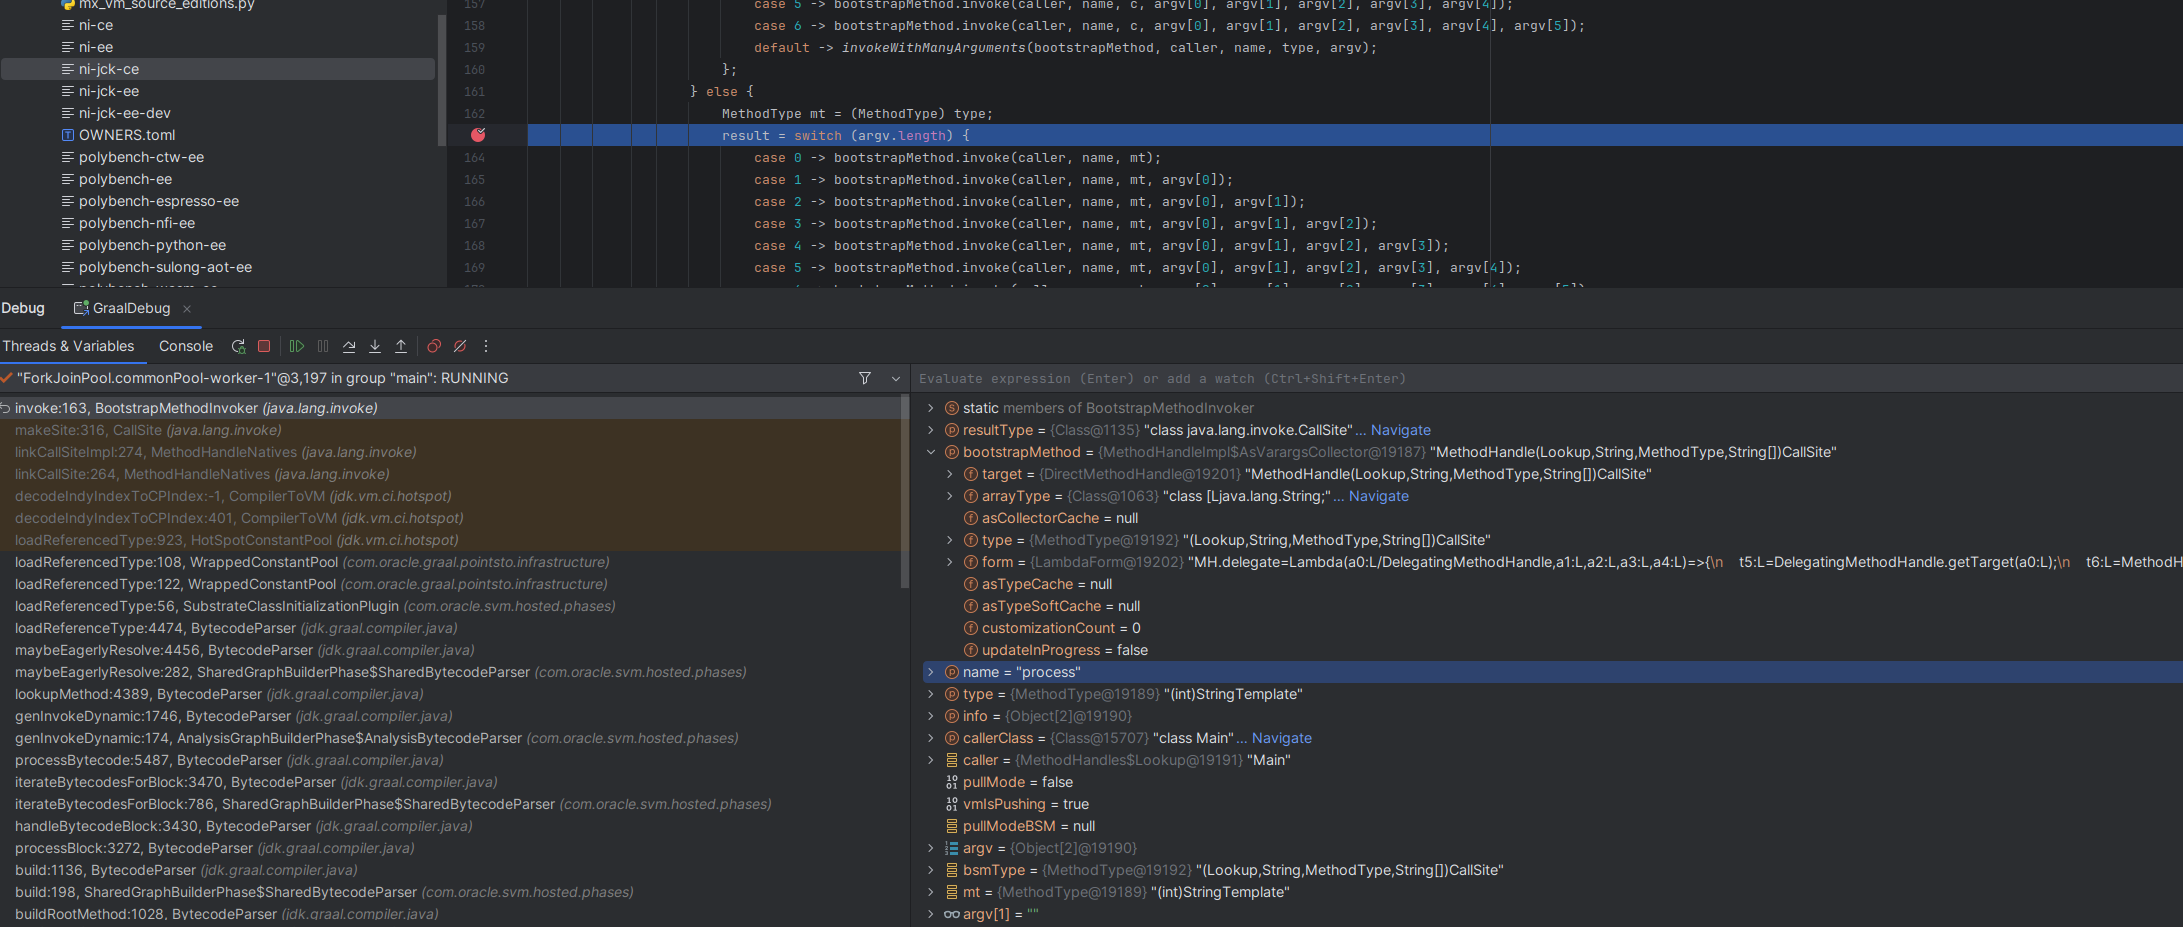
\includegraphics[width=0.5\linewidth]{resources/Screenshot from 2024-01-31 15-20-43.png}
    \caption{Enter Caption}
    \label{fig:enter-label}
\end{figure}

On StringTemplate and FormatProcessor: Added them to the indyAllowBuildTime of the BootstrapMethodConfiguration lists, i don't know why though
-> ran IGV on them nice graphs for FormatProcessor and now speedup of 3x compared to Hotspot instead of 1/2x :), for StringTemplate no speedup
-> checking that no wonky class loading is done, all LambdaForm anbd Lambda, except for this \verb|com.sun.proxy.jdk.proxy1.$Proxy76|
-> no wonky runtime exception is thrown, they get caught by the BootstrapMethodInvoker#invoke, throws a BootstrapMethodError

-> first implementation of the restrict for LambdaMetafactory and the BMI was too restrictive, i.e. only allowed LambdaMEtfactory all other bsmethod where restricted, which is not correct
-> checked NI and try to get as close as possible, it executes some safe bsmethods at build time and the rest is interpreted at runtime
-> basically only lambda and other System class are allowed in Java mode, if the user tries to do something strange (assuming they haven't overriden the App class loader), then either the call site must have been 
preloaded before, or it will throw when it tries to resolve the method name



## Define class changes

BMI#invoker
// Native Image allows certain bootstrap method to be compiled at build time as part of the
// invokedynamic instruction. In the Java mode we allow these same methods to define classes at runtime.
// We assume that all invokedynamic instructions were resolved in the step before
// program execution.
//
// @see jdk.internal.restrict.LanguageRestriction for details on language restrictions.

LambdaMetafactory#metafactory
     * Check if {@link LambdaMetafactory#metafactory} or {@link LambdaMetafactory#altMetafactory} is called
     * by {@link java.lang.invoke.BootstrapMethodInvoker} as part of an {@code invokedynamic} instruction.
     * We assume that all {@code invokedynamic} instructions were resolved in the step before
     * program execution.

ClassSpecializer#loadSpecies
// In Native Image all species code are {@code Target_java_lang_invoke_BoundMethodHandle}, as such no class resolution
// is involved. Thus, we allow calls to {@link ClassLoader#defineClass1(ClassLoader loader, String name, byte[] b, int off, int len,
// ProtectionDomain pd, String source)} even when running Java under native restrictions.
//
// @see jdk.internal.restrict.LanguageRestriction for details on language restrictions.
// @see the substitution in graal/substratevm/src/com.oracle.svm.core/src/com/oracle/svm/core/methodhandles/Target_java_lang_invoke_ClassSpecializer.java

InvokerBytecodeGenerator#loadMethod
// The method can be called form three entry points:
//    1) java.lang.invoke.InvokerBytecodeGenerator.generateCustomizedCode
//    2) java.lang.invoke.InvokerBytecodeGenerator.generateLambdaFormInterpreterEntryPoint
//    3) java.lang.invoke.InvokerBytecodeGenerator.generateNamedFunctionInvoker
// For 1) it can be proven that the LambdaForm is either customized or a MemberName is first resolved before
// the call to loadMethod is made. In Native Image, there are no calls to customize and MemberName resolution
// either involves reflection to fill the member or involves intrinsic methods.
// @see @Delete annotation on com.oracle.svm.core.methodhandles.Target_java_lang_invoke_MethodHandle#customize
// As such it is safe, in this case, for the Java mode running under native restrictions to allow class definition.
// For 2), Native Image has a substitution that always returns null, this means that all invokers are interpreted.
// @see com.oracle.svm.core.methodhandles.Target_java_lang_invoke_InvokerBytecodeGenerator#generateLambdaFormInterpreterEntryPoint
// The only method that calls 2) is LambdaForm#prepare, which also checks before if the flag to force interpretation is set.
// Native Image also has a substitution that always force interpretation.
// @see com.oracle.svm.core.methodhandles.Target_java_lang_invoke_LambdaForm#forceInterpretation
// Therefore, any calls to LambdaForm#prepare that might result in class definition in the JDK remains safe
// to execute in the Java mode under native restrictions.
// As for 3), it is called from LambdaForm#invokeWithArguments; Native Image has a substitution that does not
// compile the invoker, and thus is also safe to allow in Java.
// @see com.oracle.svm.core.methodhandles.Target_java_lang_invoke_LambdaForm_NamedFunction#invokeWithArguments
// @see com.oracle.svm.core.methodhandles.Target_java_lang_invoke_MethodHandle#invokeBasic
// @see jdk.internal.restrict.LanguageRestriction for details on language restrictions. 

MethodAccessGenerator#generate
// Under native restrictions, the generatedName must be preloaded. If the class was not preloaded, then a
// MissingReflectionRegistrationError is thrown before generate is called.
// @see jdk.internal.restrict.LanguageRestriction for details on language restrictions.
// @see substratevm/src/com.oracle.svm.core/src/com/oracle/svm/core/reflect/target/Target_java_lang_reflect_Method.java
// @see substratevm/src/com.oracle.svm.core/src/com/oracle/svm/core/reflect/target/Target_java_lang_reflect_Constructor.java
%%%%%%%%%%%%%%%%%%%%%%%%%%%%%%%%
\section{Week 20 - 05.02.24}
%%%%%%%%%%%%%%%%%%%%%%%%%%%%%%%%

Rework of the TCK, cleaning up annotation, names, and script generation

Concurrency problem on Reflection
Running Reflection JCK with:
 - Only the class checks (all class checks except for the Unsafe and array and signers and subclasses) for all checks ->

On define class:
try to minimize the amount of change -> we want one liner
Idea is in Class#loadClass public method: if Class is preloaded return the class is not then call runtimeLoadClass() and in the isClassPreloadedCheck just with tracing agent return false so that is still loads the class
Second idea is to wrap everything in lambda that calls our reflective checks -> if restrictions check fails throw else execute what's in the lambda
Last idea for define class is to check the thread lcoal in native code -> :)

%%%%%%%%%%%%%%%%%%%%%%%%%%%%%%%%
\section{Week 21 - 12.02.24}
%%%%%%%%%%%%%%%%%%%%%%%%%%%%%%%%

Hiding ThreadLocal checks with lambda:
- BMI: stack overflow
- IBG: stack overflow
- JLA: stack overflow -> moved to MethodHandles.Lookup.ClassDefiner#defineClass
- CL: in runtimeLoadClass stack overflow
- internal.Unsafe: stackOverflow


For JCK reflection with only class checks and hacks to remove Proxy\$ Lambda\$ and LambdaForm\$ java.util.stream.Collectors, in api: PASSED the second time...
java.util.MissingReflectionRegistrationError: The program tried to reflectively access class sun.util.locale.provider.SPILocaleProviderAdapter without it being registered for runtime reflection. Add sun.util.locale.provider.SPILocaleProviderAdapter to the reflection metadata to solve this problem. See https://www.graalvm.org/latest/reference-manual/native-image/metadata/#reflection for help.
	at java.base/jdk.internal.restrict.reflect.MissingReflectionRegistrationUtils.forClass(MissingReflectionRegistrationUtils.java:9)
	at java.base/jdk.internal.restrict.LanguageRestriction.checkReflectivelyAccessedClassImpl(LanguageRestriction.java:194)
	at java.base/jdk.internal.restrict.LanguageRestriction.checkReflectivelyAccessedClass(LanguageRestriction.java:184)
	at java.base/jdk.internal.restrict.reflect.ReflectiveAccessChecksImpl.checkReflectivelyAccessedClass(ReflectiveAccessChecksImpl.java:28)
	at java.base/java.lang.Class.forName(Class.java:422)
	at java.base/java.lang.Class.forName(Class.java:415)
	at java.base/sun.util.locale.provider.LocaleProviderAdapter.forType(LocaleProviderAdapter.java:193)
	at java.base/sun.util.locale.provider.LocaleProviderAdapter.findAdapter(LocaleProviderAdapter.java:293)
	at java.base/sun.util.locale.provider.LocaleProviderAdapter.getAdapter(LocaleProviderAdapter.java:264)
	at java.base/java.util.Calendar.createCalendar(Calendar.java:1696)
	at java.base/java.util.Calendar.getInstance(Calendar.java:1663)
	at java.base/java.text.SimpleDateFormat.initializeCalendar(SimpleDateFormat.java:680)
	at java.base/java.text.SimpleDateFormat.<init>(SimpleDateFormat.java:624)
	at java.base/java.text.SimpleDateFormat.<init>(SimpleDateFormat.java:579)
	at javasoft.sqe.tests.api.java.util.TreeMap.TMHdMapTests.TestCase0006(TMHdMapTests.java:300)
	at java.base/jdk.internal.reflect.DirectMethodHandleAccessor.invoke(DirectMethodHandleAccessor.java:103)
	at java.base/java.lang.reflect.Method.invoke(Method.java:581)
	at javasoft.sqe.javatest.lib.MultiTest.invokeTestCase(MultiTest.java:406)
	at javasoft.sqe.javatest.lib.MultiTest.run(MultiTest.java:195)
	at java.base/jdk.internal.reflect.DirectMethodHandleAccessor.invoke(DirectMethodHandleAccessor.java:103)
	at java.base/java.lang.reflect.Method.invoke(Method.java:581)
	at com.sun.jck.lib.ExecJCKTestSameJVMCmd$Version2Test.execute(ExecJCKTestSameJVMCmd.java:603)
	at com.sun.jck.lib.ExecJCKTestSameJVMCmd$StandardTest.run(ExecJCKTestSameJVMCmd.java:560)
	at com.sun.jck.lib.ExecJCKTestSameJVMCmd.execute(ExecJCKTestSameJVMCmd.java:444)
	at com.sun.jck.lib.ExecJCKTestSameJVMCmd.run(ExecJCKTestSameJVMCmd.java:374)
	at com.sun.javatest.agent.Agent$Task$CommandExecutor.lambda$execute$1(Agent.java:1185)
	at java.base/java.lang.Thread.run(Thread.java:1583)
TestCase0006: Failed. Test case throws exception: java.util.MissingReflectionRegistrationError: The program tried to reflectively access class sun.util.locale.provider.SPILocaleProviderAdapter without it being registered for runtime reflection. Add sun.util.locale.provider.SPILocaleProviderAdapter to the reflection metadata to solve this problem. See https://www.graalvm.org/latest/reference-manual/native-image/metadata/#reflection for help.


For defineClass
- MethodHandle.Lookup.ClassDefiner#defineClass try to fnd a way to remove that thread local
- System clean up security manager
- merge thread local into one
- create branch with just the ReflectionConfigurationParser and merge the define class branch on that instead
- looks like the linkCallsite, and loadMethod and makeInjectedInvoker are on differetn paths.

- Try to reduce scope of makeInjectedInvoker to just the Bind.bindCaller -> see where it fails in jck
- Trying to put the check in the callsite is not helpful -> they are just on the path to BMI

----------------------------------------------------------------------------------------------------------------------------------------------------------------------------------------
MethodHandleImpl#makeInjectedInvoker called not only from Bind#bindCaller but every other place that needs the CV_makeInjectedCaller#get
 IBG#LoadMethod called from 3 different places + MethodHandle#linkConstant
 BMI called from MethoHandle 2place to link
 ClassSpecializer called from same two places plus the acquireMethodAccessor
----------------------------------------------------------------------------------------------------------------------------------------------------------------------------------------

%%%%%%%%%%%%%%%%%%%%%%%%%%%%%%%%
\section{Week 22 - 19.02.24}
%%%%%%%%%%%%%%%%%%%%%%%%%%%%%%%%

Reflection
Must disable all MemberName resolution reflection check for MethodHandles, Lambdas, InjectedInvokers, LambdaNames, 

disable?
java.lang.invoke.ConstantBootstraps.staticFieldVarHandle:
Testcase "varhandle(0)" has thrown an unexpected exception java.util.MissingReflectionRegistrationError: The program tried to reflectively access field javasoft.sqe.tests.api.java.lang.invoke.ConstantBootstraps.D#z_stat_pub without it being registered for runtime reflection. Add javasoft.sqe.tests.api.java.lang.invoke.ConstantBootstraps.D#z_stat_pub to the reflection metadata to solve this problem. See https://www.graalvm.org/latest/reference-manual/native-image/metadata/#reflection for help.
java.util.MissingReflectionRegistrationError: The program tried to reflectively access field javasoft.sqe.tests.api.java.lang.invoke.ConstantBootstraps.D#z_stat_pub without it being registered for runtime reflection. Add javasoft.sqe.tests.api.java.lang.invoke.ConstantBootstraps.D#z_stat_pub to the reflection metadata to solve this problem. See https://www.graalvm.org/latest/reference-manual/native-image/metadata/#reflection for help.
        at java.base/jdk.internal.restrict.reflect.MissingReflectionRegistrationUtils.forField(MissingReflectionRegistrationUtils.java:15)
        at java.base/jdk.internal.restrict.LanguageRestriction.checkReflectivelyAccessedField(LanguageRestriction.java:269)
        at java.base/jdk.internal.restrict.LanguageRestriction.checkMethodHandleResolution(LanguageRestriction.java:279)
        at java.base/jdk.internal.restrict.reflect.ReflectiveAccessChecksImpl.memberNameResolutionCheck(ReflectiveAccessChecksImpl.java:98)
        at java.base/jdk.internal.restrict.LanguageRestrictionManager.memberNameResolutionCheck(LanguageRestrictionManager.java:369)
        at java.base/java.lang.invoke.MemberName$Factory.resolve(MemberName.java:945)
        at java.base/java.lang.invoke.MemberName$Factory.resolveOrFail(MemberName.java:994)
        at java.base/java.lang.invoke.MethodHandles$Lookup.resolveOrFail(MethodHandles.java:3745)
        at java.base/java.lang.invoke.MethodHandles$Lookup.findStaticVarHandle(MethodHandles.java:3344)
        at java.base/java.lang.invoke.ConstantBootstraps.staticFieldVarHandle(ConstantBootstraps.java:326)
        at javasoft.sqe.tests.api.java.lang.invoke.ConstantBootstraps.VarHandleTests.varhandle(VarHandleTests.java:152)
        at java.base/jdk.internal.reflect.DirectMethodHandleAccessor.invoke(DirectMethodHandleAccessor.java:103)



current exclude list
        // @see graal/substratevm/src/com.oracle.svm.configure/src/com/oracle/svm/configure/trace/AccessAdvisor.java
    static final List<String> classResolutionExcludeList = List.of(
            "java.lang.Class", // TODO check where it's used
            "java.lang.reflect.**", // TODO check where it's used
            "jdk.internal.restrict.**",
            "java.lang.invoke.DirectMethodHandle**" // NI does not compile LambdaForms -> TO remove see DirectMethodHandle l:919, 902 and 908
    );

old
            "java.lang.Class**",
            "java.lang.reflect.**",
            "jdk.internal.restrict.**",
            "java.lang.invoke.Invokers**", // NI uses another mechanism to invoke method handle that does not rely on Invokers,
            "java.lang.invoke.DirectMethodHandle**", // NI does not compile LambdaForms
            "java.lang.invoke.DelegatingMethodHandle**", // NI does not compile LambdaForms
            "java.lang.invoke.LambdaForm$Name" // NI does not compile LambdaForms


Thread Lcoal runtimedefineclass, also ignore Reflection for: 
generateConcreteSpeciesCodeCheck and generateCheck

api/java_lang/invoke/ConstantBootstraps/VarHandleTests.html -> for example of negative queries etc on reflection branch

Problem with: api/java_lang/String/FormatLocale.html for reflection branch
-> WE ALLOW RESOURCE BUNDLE SINCE IT SHOULD BE HANDLED BY RESOURCES!

%%%%%%%%%%%%%%%%%%%%%%%%%%%%%%%%
\section{Week 23 - 26.02.24}
%%%%%%%%%%%%%%%%%%%%%%%%%%%%%%%%

Restriction disable:
- Arrays#copyOf:
    - LambdaForm.BasicType: used in static final field for LambdaForm.BasicType -> probably hapens befor ethe main is initialized -> ignore
    - LambdaFormBuffer: used for LambdaFormName -> DISABLE
    - LambdaFormEditor: used for LambdaFormEditor.Transform -> DISABLE
- SharedSecrets use Class.forName to get jdk classes -> OK
- Bundles#loadBundleFromProvider -> OK
- DirectMethodHandleAccessor: for InjectedInvoker -> OK
- ServiceLoader: 
    - newInstance -> DISABLE
    - nextProviderClass -> DISABLE
    - getCosntructor -> DISABLE
- DirectMethodHandle#createFunction: for DirectMethodHandle -> DISABLE
- InvokerBytecodeGenerator#resolveFrom: for DelegatingMethodHandle\$Holder -> DISABLE
- DirectMethodHandleAccessor:
    - reflectiveInvoker: for "class\$\$InjectedInvoker" -> OK 
- MethodHandleImpl
    - getAccessor: for MethodHandleImpl.ArrayAccessor -> DISABLE, chekc if needs to be only for primitives   
    - getFunction: for MethodHandleImpl -> DISABLE
- Invokers
    - Lazy#MH_as_Spreader: for MethodHandke -> DISABLE
    - invokeBasicMethod: for MethodHandle -> DISABLE
    - getNamedFunction: for Invokers -> DISABLE
- MethodHandleNatives#makePreparedLambdaForm: for MethodHandle
- BoundMethodHandle.Specializer static inti: for BoundMethodHandle
- CallSite#getTargetHandle: for CalllSite
- DelegatingMethodHandle#makeReinvokerForm: for DelegatingMethodHandle
- DirectMethodHandle
    - makePreparedLambdaForm: for MethodHandle
    - makePreparedFieldLambdaForm: for Unsafe
- NativeMethodHandle.Lazy static init: for NativeMethodHandle
